\documentclass[12pt,letterpaper]{article}
\usepackage{fullpage}
\usepackage[top=2cm, bottom=4cm, left=2.5cm, right=2.5cm]{geometry}
\usepackage{amsmath,amsthm,amsfonts,amssymb,amscd}
\usepackage{lastpage}
\usepackage{enumerate}
\usepackage{fancyhdr}
\usepackage{mathrsfs}
\usepackage{xcolor}
\usepackage{graphicx}
\usepackage{listings}
\usepackage{hyperref}
\usepackage{float}

\hypersetup{%
  colorlinks=true,
  linkcolor=blue,
  linkbordercolor={0 0 1}
}
 
\renewcommand\lstlistingname{Algorithm}
\renewcommand\lstlistlistingname{Algorithms}
\def\lstlistingautorefname{Alg.}

\lstdefinestyle{Python}{
    language        = Python,
    frame           = lines, 
    basicstyle      = \footnotesize,
    keywordstyle    = \color{blue},
    stringstyle     = \color{green},
    commentstyle    = \color{red}\ttfamily
}

\setlength{\parindent}{0.0in}
\setlength{\parskip}{0.05in}
\begin{document}

\begin{enumerate}
    \item \emph{Solution.}
    \begin{enumerate}
      \item As $x$ gets smaller and smaller, we see that the reformulated equation 
      does much better than the original estimation. In fact, the original estimation
      seems to float around the actual value and then, because of loss of significance, 
      seems to think that the numerator is so small, it is just zero. \\
      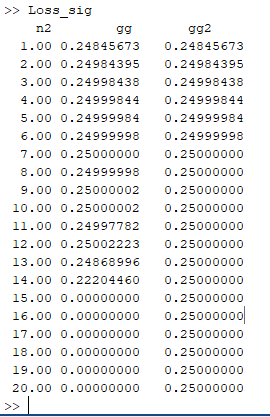
\includegraphics{loss_sig a.png}

      \item Here, as x gets smaller, we see that the original does quite well but again, 
      the numerator loses much significance which the computer assumes is zero. \\
      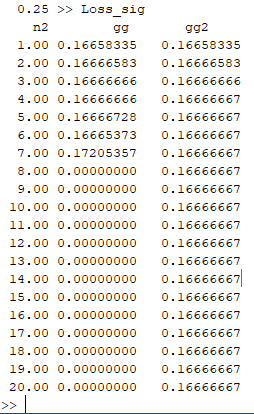
\includegraphics{loss_sig b.png}
    \end{enumerate}

    \item \emph{Solution.} 
    \begin{enumerate}
      \item For our approximation for $\pi$ (22/7): \\
      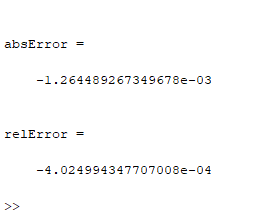
\includegraphics{pi error.png}
      \item For our approximation for $e$ (2.718): \\
      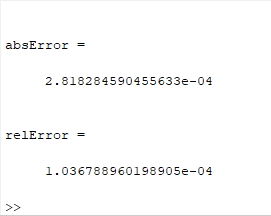
\includegraphics{exp error .png}
      \item For our approximation for $\sqrt{2}$ (1.414): \\
      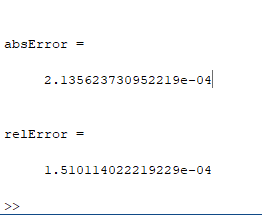
\includegraphics{root2 error.png}
    \end{enumerate}

    \item \emph{Solution.}
    \begin{enumerate}
      \item 
      \begin{gather}
        \frac{|p^* - \pi|}{|\pi|} \leq .0001 \\
        |p^* - \pi| \leq .0001\pi
      \end{gather}
      Applying absolute value: 
      \begin{gather}
        -.0001\pi \leq p^*-\pi \leq .0001\pi \\
        -.0001\pi + \pi \leq p^* \leq .0001\pi + \pi\\
        .9999\pi \leq p^* \leq 1.0001\pi
      \end{gather}

      Therefore, our $p^*$ value must be in the interval $(.9999\pi,1.0001\pi)$
      \item 
      \begin{gather}
        \frac{|p^* - e|}{|e|} = .0001 \\
        |p^* - e| \leq .0001e
      \end{gather}
      Applying absolute value: 
      \begin{gather}
        -.0001e \leq p^*-e \leq .0001e \\
        -.0001e+ e \leq p^* \leq .0001e + e\\
        .9999e \leq p^* \leq 1.0001e
      \end{gather}

      Therefore, our $p^*$ value must be in the interval $(.9999e,1.0001e)$
      \item 
      \begin{gather}
        \frac{|p^* - \sqrt{2}|}{|\sqrt{2}|} = .0001 \\
        |p^* - \sqrt{2}| \leq .0001\sqrt{2}
      \end{gather}
      Applying absolute value: 
      \begin{gather}
        -.0001\sqrt{2} \leq p^*-\sqrt{2} \leq .0001\sqrt{2} \\
        -.0001\sqrt{2}+ \sqrt{2} \leq p^* \leq .0001\sqrt{2} + \sqrt{2}\\
        .9999\sqrt{2} \leq p^* \leq 1.0001\sqrt{2}
      \end{gather}

      Therefore, our $p^*$ value must be in the interval $(.9999\sqrt{2},1.0001\sqrt{2})$
    \end{enumerate}

    \item Using the nest.m function and the equivalent expression, we see that the 
    two values are slightly different: \\
    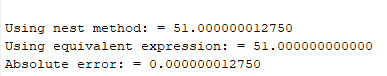
\includegraphics{number4.png}
\end{enumerate}

\end{document}